% 12pt .6pt grayscale native fragment
\usetikzlibrary{calc}
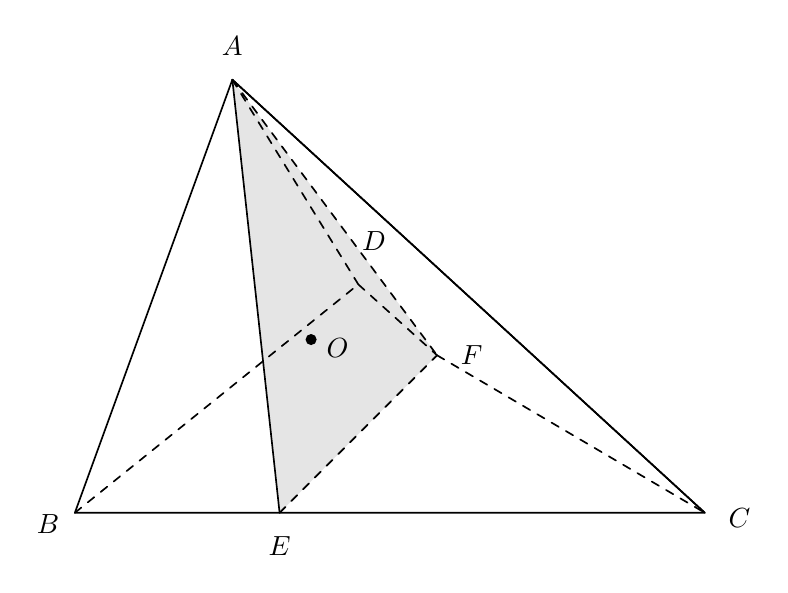
\begin{tikzpicture}[line width=0.6pt, line join=round, line cap=round, >=stealth]
\tikzset{hid/.style={dashed}}
\coordinate (A) at (2,5.5); \coordinate (B) at (0,0); \coordinate (C) at (8,0); \coordinate (E) at (2.6,0); \coordinate (F) at (4.6,2.0); \coordinate (D) at (3.6,2.9); \coordinate (O) at (3.0,2.2);
\fill[gray!20] (A)--(F)--(E)--cycle;
\draw (A)--(B)--(C)--cycle; \draw (A)--(C); \draw (A)--(E); \draw[hid] (E)--(F); \draw[hid] (F)--(C); \draw[hid] (B)--(D); \draw[hid] (D)--(F); \draw[hid] (A)--(D); \draw[hid] (A)--(F);
\fill (O) circle (2pt);
\node[above=5pt] at (A) {$A$}; \node[below=4pt,left=2pt] at (B) {$B$}; \node[below=2pt,right=5pt] at (C) {$C$};
\node[below=5pt] at (E) {$E$}; \node[right=5pt] at (F) {$F$}; \node at (3.8,3.45) {$D$}; \node[below=3pt,right=2pt] at (O) {$O$};
\end{tikzpicture}
